\documentclass[10.5pt,a4paper]{article}

\usepackage[a4paper,top=2.0cm,bottom=1.9cm,left=1.9cm,right=1.9cm]{geometry}
\usepackage{amsmath,amssymb,mathtools}
\usepackage[T1]{fontenc}
\usepackage{lmodern}
\usepackage{microtype}
\usepackage[table]{xcolor}
\usepackage{booktabs}
\usepackage{tabularx}
\usepackage{array}
\usepackage{enumitem}
\usepackage{titlesec}
\usepackage{fancyhdr}
\usepackage[most]{tcolorbox}
\usepackage{lastpage}
\usepackage{tikz}
\usetikzlibrary{arrows.meta}
\usepackage[hidelinks]{hyperref}

\definecolor{navy}{HTML}{1F3A5F}
\definecolor{teal}{HTML}{0F6E6E}
\definecolor{violet}{HTML}{5B3A8E}
\definecolor{rust}{HTML}{B45309}
\definecolor{accent}{named}{navy}

\pagestyle{fancy}
\fancyhf{}
\fancyhead[L]{\small\color{black!65}Numerical Methods --- Master Revision}
\fancyhead[R]{\small\color{black!65}\leftmark}
\fancyfoot[C]{\small\color{black!65}\thepage\ / \pageref{LastPage}}
\renewcommand{\headrulewidth}{0.3pt}
\renewcommand{\headrule}{\hbox to\headwidth{\color{accent!40}\leaders\hrule height \headrulewidth\hfill}}

\titleformat{\section}
  {\Large\bfseries\color{accent}}
  {\thesection}{0.6em}{}
  [{\vspace{-0.2em}\color{accent}\rule{\linewidth}{0.9pt}}]
\titleformat{\subsection}
  {\large\bfseries\color{accent!90!black}}
  {\thesubsection}{0.5em}{}
\titlespacing*{\section}{0pt}{10pt}{5pt}
\titlespacing*{\subsection}{0pt}{7pt}{3pt}

\setlength{\parindent}{0pt}
\setlength{\parskip}{3.5pt}
\setlength{\abovedisplayskip}{4pt}
\setlength{\belowdisplayskip}{4pt}
\setlist[itemize]{leftmargin=1.2em,itemsep=1pt,topsep=2pt}
\setlist[enumerate]{leftmargin=1.5em,itemsep=1pt,topsep=2pt}
\renewcommand{\arraystretch}{1.18}

\newtcolorbox{keybox}[1][Key result]{
  enhanced, breakable,
  colback=accent!4, colframe=accent!80!black,
  boxrule=0.7pt, arc=1.4mm,
  left=5pt,right=5pt,top=3pt,bottom=3pt,
  title={#1}, fonttitle=\small\bfseries,
  coltitle=white, colbacktitle=accent!80!black
}
\newtcolorbox{derivbox}[1][Derivation]{
  enhanced, breakable,
  colback=black!3, colframe=black!38,
  boxrule=0.5pt, arc=1mm,
  left=5pt,right=5pt,top=3pt,bottom=3pt,
  title={#1}, fonttitle=\small\bfseries,
  coltitle=black, colbacktitle=black!9
}
\newtcolorbox{warnbox}[1][Watch out]{
  enhanced, breakable,
  colback=rust!5, colframe=rust!75!black,
  boxrule=0.6pt, arc=1mm,
  left=5pt,right=5pt,top=3pt,bottom=3pt,
  title={#1}, fonttitle=\small\bfseries,
  coltitle=white, colbacktitle=rust!80!black
}
\newtcolorbox{overviewbox}[2][]{
  enhanced, colback=#1!5, colframe=#1!80!black,
  boxrule=0.6pt, arc=1.2mm,
  left=5pt,right=5pt,top=3pt,bottom=3pt,
  title={#2}, fonttitle=\small\bfseries,
  coltitle=white, colbacktitle=#1!80!black
}

\newcommand{\dd}{\mathrm{d}}
\newcommand{\x}{\mathbf{x}}
\newcommand{\R}{\mathbb{R}}
\newcommand{\avg}[1]{\left\langle #1 \right\rangle}

\begin{document}

%============================================================
% TITLE + COURSE MAP
%============================================================
\begin{center}
{\color{navy}\rule{\linewidth}{2pt}}\\[0.5em]
{\Huge\bfseries Numerical Methods}\\[16pt]
{\LARGE Master Revision Guide}\\[8pt]
{\large Linear \& Nonlinear ODEs \quad$\cdot$\quad Linear PDEs \quad$\cdot$\quad Stochastic Systems}\\[3pt]
{\small Phy 324 --- distilled from the handwritten notes and the NotebookLM mind map}\\[0.4em]
{\color{navy}\rule{\linewidth}{2pt}}
\end{center}

\vspace{0.2em}
{\color{navy}\Large\bfseries The whole course on one page}

\vspace{0.3em}
\noindent
\begin{minipage}[t]{0.487\textwidth}
\begin{overviewbox}[navy]{Linear ODEs}
\begin{itemize}
\item Euler and improved Euler
\item Explicit vs implicit methods
\item Stability and step-size limits
\item Decay: $N=N_0e^{-\lambda t}$
\item Oscillator: $m\ddot x+\gamma\dot x+kx=0$
\end{itemize}
\end{overviewbox}
\vspace{0.2em}
\begin{overviewbox}[navy]{Nonlinear ODEs}
\begin{itemize}
\item Steady states: $f(x^*)=0$
\item Linearise: use $f'(x^*)$
\item 2D: Jacobian eigenvalues
\item Double well and rotating hoop
\end{itemize}
\end{overviewbox}
\end{minipage}\hfill
\begin{minipage}[t]{0.487\textwidth}
\begin{overviewbox}[violet]{Linear PDEs}
\begin{itemize}
\item Diffusion: $\rho_t=D\rho_{xx}$
\item Wave: $\psi_{tt}=c^2\psi_{xx}$
\item Finite differences on a grid
\item von Neumann: $D\Delta t/\Delta x^2\le\frac12$
\item CFL: $c\Delta t/\Delta x\le1$
\end{itemize}
\end{overviewbox}
\vspace{0.2em}
\begin{overviewbox}[rust]{Stochastic Systems}
\begin{itemize}
\item Brownian motion: Langevin equation
\item Noise: mean zero, delta-correlated
\item Random walk: $\avg{x_n^2}=na^2$
\item Diffusion limit: $D=a^2/(2\Delta t)$
\end{itemize}
\end{overviewbox}
\end{minipage}

\vspace{0.6em}
\begin{keybox}[Notation and the one idea behind everything]
\[
t_n=t_0+nh,\qquad y_n\approx y(t_n),\qquad x_i=i\Delta x,\qquad
L=N\Delta x.
\]
A derivative is replaced by a finite difference, a PDE becomes a set of
algebraic update rules, and the two questions are always:
\textbf{(i) how accurate is it?} (order) and
\textbf{(ii) does the error grow?} (stability).
\end{keybox}

\vspace{0.4em}
\begin{keybox}[Roadmap]
\begin{itemize}
\item \textbf{Part 1 --- Linear ODEs:} exact solution of the test equation,
Euler, improved Euler, explicit vs implicit, the damped oscillator.
\item \textbf{Part 2 --- Nonlinear ODEs:} fixed points, linearisation,
the Jacobian classification, the double well and the rotating hoop.
\item \textbf{Part 3 --- Linear PDEs:} diffusion from Fick's law, the wave
equation, finite differences, von Neumann/CFL, boundary conditions.
\item \textbf{Part 4 --- Stochastic systems:} Langevin equation,
mean squared displacement, random walk and its diffusion limit.
\end{itemize}
\end{keybox}

%============================================================
\clearpage
\colorlet{accent}{navy}
\section{Linear Ordinary Differential Equations}

\subsection{The model problem and exact solutions}

A first-order linear ODE has the form
\[
y'+p(t)y=q(t).
\]
The integrating factor is \(\mu(t)=e^{\int p(t)\dd t}\), because
\((\mu y)'=\mu q\). Hence
\[
y(t)=\frac{1}{\mu(t)}\left(C+\int \mu(t)q(t)\dd t\right).
\]

The most important special case is the \emph{decay equation}
\[
\boxed{\;y'=-\lambda y\quad\Longrightarrow\quad y(t)=y(0)e^{-\lambda t}\;}
\qquad \tau=\frac{1}{\lambda}.
\]
\(\tau\) is the characteristic time scale: after time \(\tau\) the
solution has fallen by a factor \(e\).

\begin{keybox}[Nuclear decay]
\[
\frac{\dd N}{\dd t}=-\lambda N
\quad\Longrightarrow\quad
N(t)=N_0e^{-\lambda t},
\qquad
t_{1/2}=\frac{\ln 2}{\lambda}.
\]
The decay equation is also the standard \emph{test equation} for
stability: every numerical method is analysed on \(y'=-\lambda y\),
\(\lambda>0\).
\end{keybox}

\subsection{Euler's method}

\begin{derivbox}[Derivation: forward difference]
Taylor expand the exact solution:
\[
y(t+h)=y(t)+h y'(t)+\frac{h^2}{2}y''(c).
\]
Use \(y'=f(t,y)\) and drop the \(O(h^2)\) remainder:
\[
y(t+h)\approx y(t)+h f(t,y(t)).
\]
This gives the explicit Euler update.
\end{derivbox}

\begin{keybox}[Explicit Euler]
\[
y_{n+1}=y_n+h f(t_n,y_n).
\]
\textbf{Local error:} \(O(h^2)\).\quad
\textbf{Global error:} \(O(h)\) (first order).
\end{keybox}

\textbf{Why the global order drops.} In one step the error is
\(\tau_n\approx \frac{h^2}{2}y''(c)=O(h^2)\). After \(N=T/h\) steps the
errors accumulate:
\[
\text{global error}\approx N\cdot O(h^2)
=\frac{T}{h}O(h^2)=O(h).
\]

\begin{derivbox}[Stability on \(y'=-\lambda y\)]
\[
y_{n+1}=y_n-\lambda h\,y_n=(1-\lambda h)y_n
\quad\Longrightarrow\quad
y_n=(1-\lambda h)^n y_0.
\]
The numerical solution decays only if
\[
|1-\lambda h|\le1
\quad\Longleftrightarrow\quad
0\le \lambda h\le2
\quad\Longleftrightarrow\quad
h\le\frac{2}{\lambda}.
\]
\end{derivbox}

\begin{keybox}[Euler stability and step size]
\[
\boxed{\;h\le\frac{2}{\lambda}\;}
\]
\begin{itemize}
\item \(h<1/\lambda\): smooth monotone decay (the stricter, positivity-preserving choice).
\item \(1/\lambda<h<2/\lambda\): decaying but oscillating sign.
\item \(h>2/\lambda\): numerical blow-up.
\end{itemize}
\end{keybox}

\subsection{Improved Euler (Heun's predictor--corrector)}

\begin{derivbox}[Derivation: trapezoidal rule]
Integrate the ODE exactly over one step:
\[
y_{n+1}=y_n+\int_{t_n}^{t_{n+1}}f(t,y)\dd t.
\]
Approximate the integral by the trapezoidal rule:
\[
y_{n+1}=y_n+\frac{h}{2}\left[f_n+f_{n+1}\right].
\]
The unknown \(f_{n+1}\) is estimated with a predicted value
\(y_p=y_n+hf_n\). This gives the improved Euler method.
\end{derivbox}

\begin{keybox}[Improved Euler]
\[
y_p=y_n+h f(t_n,y_n),
\]
\[
y_{n+1}=y_n+\frac{h}{2}\left[f(t_n,y_n)+f(t_{n+1},y_p)\right].
\]
\textbf{Local error:} \(O(h^3)\).\quad
\textbf{Global error:} \(O(h^2)\) (second order).
\end{keybox}

\begin{derivbox}[Stability]
On \(y'=-\lambda y\), put \(z=\lambda h\):
\[
y_{n+1}=\left(1-z+\frac{z^2}{2}\right)y_n.
\]
The polynomial \(P(z)=1-z+z^2/2\) satisfies \(|P(z)|\le1\) for
\(0\le z\le2\). Hence
\[
h\le\frac{2}{\lambda}.
\]
\end{derivbox}

\subsection{Explicit vs implicit methods}

\begin{center}
\begin{tabularx}{\linewidth}{@{}>{\raggedright\arraybackslash}p{0.18\linewidth}
  >{\raggedright\arraybackslash}X
  >{\centering\arraybackslash}p{0.10\linewidth}
  >{\raggedright\arraybackslash}p{0.24\linewidth}@{}}
\toprule
\rowcolor{accent!10}
\textbf{Method} & \textbf{Update} & \textbf{Order} & \textbf{Stability} \\
\midrule
Explicit Euler & \(y_{n+1}=y_n+hf(t_n,y_n)\) & 1 &
\(h\le2/\lambda\); cheap, conditionally stable \\
Implicit Euler & \(y_{n+1}=y_n+hf(t_{n+1},y_{n+1})\) & 1 &
unconditionally stable for \(\lambda>0\); needs a solve \\
\bottomrule
\end{tabularx}
\end{center}

For the linear test equation, implicit Euler gives
\[
y_{n+1}=\frac{y_n}{1+\lambda h},
\qquad
\left|\frac{1}{1+\lambda h}\right|\le1
\quad\text{for all }h>0.
\]
That is why stiff problems prefer implicit methods.

\subsection{Harmonic oscillator}

For a damped spring,
\[
m\ddot x+\gamma\dot x+kx=0.
\]
Divide by \(m\) and define
\[
b=\frac{\gamma}{2m},\qquad \omega_0=\sqrt{\frac{k}{m}}.
\]
Then
\[
\ddot x+2b\dot x+\omega_0^2x=0.
\]
Substituting \(x=e^{rt}\) gives the characteristic equation
\[
r^2+2br+\omega_0^2=0
\quad\Longrightarrow\quad
r=-b\pm\sqrt{b^2-\omega_0^2}.
\]

\begin{center}
\begin{tabularx}{\linewidth}{@{}>{\raggedright\arraybackslash}p{0.17\linewidth}
  >{\centering\arraybackslash}p{0.17\linewidth}
  >{\raggedright\arraybackslash}X@{}}
\toprule
\rowcolor{accent!10}
\textbf{Regime} & \textbf{Condition} & \textbf{Solution} \\
\midrule
Underdamped & \(b^2<\omega_0^2\) &
\(x=e^{-bt}(A\cos\omega_d t+B\sin\omega_d t)\),
\(\omega_d=\sqrt{\omega_0^2-b^2}\) \\
Critically damped & \(b^2=\omega_0^2\) &
\(x=(A+Bt)e^{-bt}\) \\
Overdamped & \(b^2>\omega_0^2\) &
\(x=Ae^{r_1t}+Be^{r_2t}\), \(r_{1,2}=-b\pm\sqrt{b^2-\omega_0^2}\) \\
\bottomrule
\end{tabularx}
\end{center}

\begin{keybox}[What the regimes mean]
\begin{itemize}
\item \textbf{Underdamped:} oscillates with a decaying envelope.
\item \textbf{Critically damped:} returns to equilibrium as fast as possible without oscillating.
\item \textbf{Overdamped:} returns slowly, without oscillating.
\end{itemize}
The imaginary part of \(r\) gives oscillation; the real part \(-b\) gives decay.
\end{keybox}

\subsection{Damping ratio and energy}

It is useful to write the damping as a dimensionless number:
\[
\zeta=\frac{b}{\omega_0}
=\frac{\gamma}{2\sqrt{km}}.
\]
Then
\[
\zeta<1:\ \text{underdamped},\qquad
\zeta=1:\ \text{critically damped},\qquad
\zeta>1:\ \text{overdamped}.
\]

\begin{derivbox}[Energy decreases]
The mechanical energy is
\[
E=\frac12m\dot x^2+\frac12kx^2.
\]
Differentiate and use \(m\ddot x=-\gamma\dot x-kx\):
\[
\frac{\dd E}{\dd t}
=m\dot x\ddot x+kx\dot x
=\dot x\,(m\ddot x+kx)
=-\gamma\dot x^2\le0.
\]
So damping always removes energy; it never adds energy.
\end{derivbox}

\begin{center}
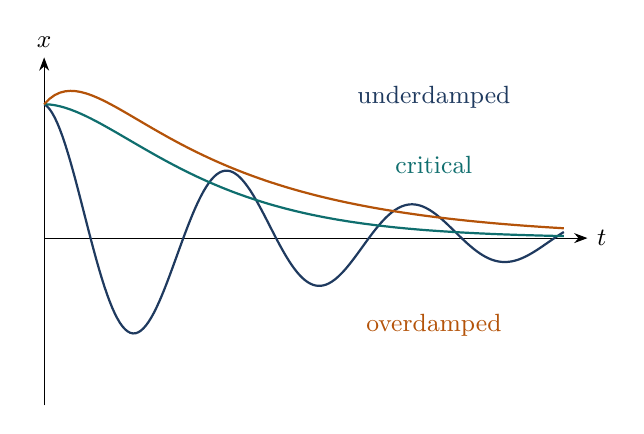
\begin{tikzpicture}[x=0.75cm,y=1.7cm,>=Stealth]
  \draw[->] (0,0)--(9.2,0) node[right] {\small $t$};
  \draw[->] (0,-1.25)--(0,1.35) node[above] {\small $x$};
  \draw[thick,navy,domain=0:8.8,samples=200]
    plot (\x,{exp(-0.22*\x)*cos(2*\x r)});
  \draw[thick,teal,domain=0:8.8,samples=100]
    plot (\x,{(1+0.7*\x)*exp(-0.7*\x)});
  \draw[thick,rust,domain=0:8.8,samples=100]
    plot (\x,{1.6*exp(-0.35*\x)-0.6*exp(-1.8*\x)});
  \node[navy] at (6.6,1.05) {\small underdamped};
  \node[teal] at (6.6,0.55) {\small critical};
  \node[rust] at (6.6,-0.65) {\small overdamped};
\end{tikzpicture}
\end{center}

%============================================================
\clearpage
\colorlet{accent}{teal}
\section{Nonlinear Ordinary Differential Equations}

\subsection{Fixed points and linear stability}

A one-dimensional autonomous system is
\[
\dot x=f(x).
\]
A \emph{steady state} or \emph{fixed point} \(x^*\) satisfies
\[
f(x^*)=0.
\]

\begin{derivbox}[Derivation: linearisation]
Perturb the fixed point: \(x=x^*+u\), with \(u\) small. Taylor expand:
\[
f(x^*+u)=\underbrace{f(x^*)}_{=0}+f'(x^*)\,u
+\frac{f''(x^*)}{2}u^2+\cdots
\]
Since \(f(x^*)=0\), the linear term gives
\[
\dot u=f'(x^*)\,u.
\]
Therefore
\[
u(t)=u(0)e^{f'(x^*)t}.
\]
\end{derivbox}

\begin{keybox}[Stability criterion in 1D]
\[
\boxed{f'(x^*)<0\ \Longrightarrow\ \text{stable},\qquad
f'(x^*)>0\ \Longrightarrow\ \text{unstable}.}
\]
If \(f'(x^*)=0\), the linear test is inconclusive and one must look at
higher derivatives or the graph.
\end{keybox}

\textbf{Graphical analysis.} Plot \(f(x)\) against \(x\).
\begin{itemize}
\item Zeros of \(f\) are fixed points.
\item Where \(f>0\), the state moves right; where \(f<0\), it moves left.
\item Arrows pointing towards a fixed point mean stable; away means unstable.
\end{itemize}

\begin{keybox}[Example: logistic growth]
\[
\dot x=x(1-x).
\]
Fixed points: \(x^*=0,1\).
\[
f'(x)=1-2x
\quad\Longrightarrow\quad
f'(0)=1>0\ \text{(unstable)},\quad
f'(1)=-1<0\ \text{(stable)}.
\]
\end{keybox}

\subsection{Double-well potential}

A clean nonlinear example is the damped gradient flow
\[
\dot x=-V'(x).
\]
The standard double well is
\[
V(x)=-\frac{k}{2}x^2+\frac{\lambda}{4}x^4
\qquad(k,\lambda>0).
\]
Then
\[
V'(x)=-kx+\lambda x^3,
\]
so
\[
\dot x=kx-\lambda x^3=x(k-\lambda x^2).
\]
Fixed points:
\[
x^*=0,\qquad x^*=\pm\sqrt{\frac{k}{\lambda}}.
\]
Linear stability:
\[
f'(x)=k-3\lambda x^2,
\]
so
\[
f'(0)=k>0\ \text{(unstable)},\qquad
f'\!\left(\pm\sqrt{k/\lambda}\right)=-2k<0\ \text{(stable)}.
\]

\begin{warnbox}[Sign check]
The mind map writes \(V=\frac12kx^2-\frac14\lambda x^4\). With positive
\(k,\lambda\) that is an \emph{inverted} well: the minimum is at \(0\),
not at \(\pm\sqrt{k/\lambda}\). For the usual double well, the quadratic
term must be negative, as above.
\end{warnbox}

\subsection{Two-dimensional linear systems}

For
\[
\dot x=ax+by,\qquad \dot y=cx+dy,
\]
write
\[
\dot{\x}=J\x,\qquad
J=\begin{bmatrix}a&b\\c&d\end{bmatrix}.
\]
Substituting \(\x=\mathbf v e^{\lambda t}\) gives
\[
J\mathbf v=\lambda\mathbf v
\quad\Longrightarrow\quad
\det(J-\lambda I)=0.
\]
Thus
\[
\lambda^2-\tau\lambda+\Delta=0,
\qquad
\tau=\operatorname{tr}J=a+d,\quad
\Delta=\det J=ad-bc.
\]
The general solution is
\[
\x(t)=\alpha\mathbf v_1e^{\lambda_1t}+\beta\mathbf v_2e^{\lambda_2t}.
\]
The fixed point is stable exactly when
\[
\operatorname{Re}\lambda_1<0\quad\text{and}\quad \operatorname{Re}\lambda_2<0.
\]

\begin{center}
\begin{tabularx}{\linewidth}{@{}>{\centering\arraybackslash}p{0.10\linewidth}
  >{\centering\arraybackslash}p{0.10\linewidth}
  >{\centering\arraybackslash}p{0.15\linewidth}
  >{\raggedright\arraybackslash}X@{}}
\toprule
\rowcolor{accent!10}
\(\Delta\) & \(\tau\) & Discriminant & Type of fixed point \\
\midrule
\(<0\) & any & any & saddle (one eigenvalue positive, one negative) \\
\(>0\) & \(<0\) & \(\tau^2-4\Delta>0\) & stable node \\
\(>0\) & \(<0\) & \(\tau^2-4\Delta<0\) & stable spiral \\
\(>0\) & \(>0\) & \(\tau^2-4\Delta>0\) & unstable node \\
\(>0\) & \(>0\) & \(\tau^2-4\Delta<0\) & unstable spiral \\
\(>0\) & \(0\) & \(\tau^2-4\Delta<0\) & centre (neutral oscillation) \\
\bottomrule
\end{tabularx}
\end{center}

\begin{keybox}[Quick classification]
\[
\Delta<0:\ \text{saddle},
\qquad
\Delta>0,\ \tau<0:\ \text{stable},
\qquad
\Delta>0,\ \tau>0:\ \text{unstable}.
\]
If \(\Delta>0\), the discriminant \(\tau^2-4\Delta\) decides
\emph{node} (positive) versus \emph{spiral} (negative).
\end{keybox}

\subsection{Bead on a rotating hoop}

A hoop of radius \(R\) rotates about a vertical diameter with angular
speed \(\Omega\). Let \(\phi\) be the bead's angle measured from the
bottom. The tangential forces are:
\begin{itemize}
\item gravity: \(-mg\sin\phi\),
\item centrifugal: \(+mR\Omega^2\sin\phi\cos\phi\),
\item damping: \(-bR\dot\phi\).
\end{itemize}
Hence
\[
mR\ddot\phi=-bR\dot\phi-mg\sin\phi+mR\Omega^2\sin\phi\cos\phi.
\]
Divide by \(mR\):
\[
\ddot\phi=-\frac{b}{m}\dot\phi-\frac{g}{R}\sin\phi
+\Omega^2\sin\phi\cos\phi.
\]

\textbf{Fixed points.} Set \(\dot\phi=\ddot\phi=0\):
\[
\sin\phi\left(\Omega^2\cos\phi-\frac{g}{R}\right)=0.
\]
Therefore
\[
\phi^*=0,\ \pi,
\qquad\text{and, if }\Omega^2>\frac{g}{R},\quad
\phi^*=\pm\arccos\!\left(\frac{g}{R\Omega^2}\right).
\]

\begin{keybox}[Pitchfork bifurcation]
The critical speed is
\[
\Omega_c^2=\frac{g}{R}.
\]
\begin{itemize}
\item \(\Omega^2<\Omega_c^2\): only \(\phi=0\) is stable (bead at the bottom).
\item \(\Omega^2>\Omega_c^2\): \(\phi=0\) becomes unstable and the two symmetric
points \(\pm\phi^*\) are stable.
\end{itemize}
This is a pitchfork bifurcation.
\end{keybox}

\subsubsection*{Why the new fixed points are stable}

Write the right-hand side of the angle equation as
\[
g(\phi)=-\frac{g}{R}\sin\phi+\Omega^2\sin\phi\cos\phi.
\]
Then
\[
g'(\phi)=-\frac{g}{R}\cos\phi
+\Omega^2(\cos^2\phi-\sin^2\phi).
\]
At the bottom,
\[
g'(0)=\Omega^2-\frac{g}{R}.
\]
Thus \(\phi=0\) is stable for \(\Omega^2<g/R\) and unstable for
\(\Omega^2>g/R\).
At the nontrivial fixed point, \(\cos\phi^*=g/(R\Omega^2)\), and
\[
g'(\phi^*)=-\Omega^2\sin^2\phi^*<0,
\]
so the two symmetric points are stable. The stability switch at
\(\Omega_c^2=g/R\) is exactly the pitchfork.

\begin{center}
\begin{tikzpicture}[x=1.35cm,y=1.15cm,>=Stealth]
  \draw[->] (0,0)--(6.5,0) node[right] {\small $\Omega^2$};
  \draw[->] (0,-2.4)--(0,2.5) node[above] {\small $\phi^*$};
  \draw[very thick,teal] (0,0)--(3,0);
  \draw[thick,dashed,teal] (3,0)--(6.2,0);
  \draw[very thick,rust] (3,0) to[out=18,in=200] (6.2,1.9);
  \draw[very thick,rust] (3,0) to[out=-18,in=160] (6.2,-1.9);
  \draw[dashed] (3,-0.15)--(3,0.15);
  \node[below] at (3,-0.12) {\small $\Omega_c^2=g/R$};
  \node[teal] at (1.45,0.32) {\small stable};
  \node[teal] at (4.6,-0.32) {\small unstable};
  \node[rust] at (4.7,1.55) {\small stable $\pm\phi^*$};
\end{tikzpicture}
\end{center}

\subsubsection*{Effective potential}

There is a compact way to see the same result. Define the effective
potential
\[
V_{\text{eff}}(\phi)
=-mgR\cos\phi-\frac12mR^2\Omega^2\sin^2\phi.
\]
Then
\[
V_{\text{eff}}'(\phi)
=mgR\sin\phi-mR^2\Omega^2\sin\phi\cos\phi
=-mR^2g(\phi).
\]
Fixed points are extrema of \(V_{\text{eff}}\), and minima are stable.
At \(\Omega^2<g/R\), the bottom \(\phi=0\) is the minimum. At
\(\Omega^2>g/R\), the bottom becomes a maximum and two symmetric minima
appear at \(\pm\phi^*\). This is precisely the pitchfork shown above.

%============================================================
\clearpage
\colorlet{accent}{violet}
\section{Linear Partial Differential Equations}

\subsection{Diffusion equation}

Let \(\rho(x,t)\) be a density and \(J(x,t)\) the flux. Conservation of
particles reads
\[
\frac{\partial\rho}{\partial t}+\frac{\partial J}{\partial x}=0.
\]
Fick's law says the flux is proportional to the negative gradient:
\[
J=-D\frac{\partial\rho}{\partial x}.
\]

\begin{derivbox}[Derivation of the diffusion equation]
Substitute Fick's law into continuity:
\[
\frac{\partial\rho}{\partial t}
=-\frac{\partial J}{\partial x}
=\frac{\partial}{\partial x}
\left(D\frac{\partial\rho}{\partial x}\right).
\]
For constant \(D\),
\[
\boxed{\;\frac{\partial\rho}{\partial t}
=D\frac{\partial^2\rho}{\partial x^2}\;}
\]
In three dimensions,
\(\partial_t\rho=D\nabla^2\rho\).
\end{derivbox}

\begin{keybox}[Diffusion facts]
\begin{itemize}
\item Steady state: \(\nabla^2\rho=0\) (Laplace equation).
\item Initial spike spreads as a Gaussian:
\[
\rho(x,t)=\frac{1}{\sqrt{4\pi Dt}}
\exp\!\left(-\frac{x^2}{4Dt}\right).
\]
\item Mean squared displacement: \(\avg{x^2}=2Dt\) in 1D.
\end{itemize}
\end{keybox}

\subsection{Wave equation}

The second-order wave equation is
\[
\frac{\partial^2\psi}{\partial t^2}
=c^2\frac{\partial^2\psi}{\partial x^2}.
\]

\begin{derivbox}[Derivation: factor the operator]
\[
\left(\frac{\partial}{\partial t}-c\frac{\partial}{\partial x}\right)
\left(\frac{\partial}{\partial t}+c\frac{\partial}{\partial x}\right)\psi
=
\frac{\partial^2\psi}{\partial t^2}
-c^2\frac{\partial^2\psi}{\partial x^2}
=0.
\]
So the equation is satisfied by a sum of a right-moving and a
left-moving wave:
\[
\boxed{\;\psi(x,t)=f(x-ct)+g(x+ct)\;}
\]
\end{derivbox}

\begin{keybox}[One-way waves]
A right-moving pulse \(f(x-ct)\) satisfies the first-order equation
\[
\frac{\partial\psi}{\partial t}
=-c\frac{\partial\psi}{\partial x}.
\]
A left-moving pulse satisfies
\(\partial_t\psi=+c\partial_x\psi\).
The first-order advection equation keeps only one direction; the
second-order equation keeps both.
\end{keybox}

\subsection{Finite differences}

Put the grid points at
\[
x_i=i\Delta x,\qquad i=0,1,\dots,N,\qquad L=N\Delta x.
\]
Taylor expansion gives
\[
f(x_{i+1})=f_i+\Delta x f_i'
+\frac{\Delta x^2}{2}f_i''
+\frac{\Delta x^3}{6}f_i'''+\cdots
\]
\[
f(x_{i-1})=f_i-\Delta x f_i'
+\frac{\Delta x^2}{2}f_i''
-\frac{\Delta x^3}{6}f_i'''+\cdots
\]

\begin{center}
\begin{tabularx}{\linewidth}{@{}>{\raggedright\arraybackslash}p{0.20\linewidth}
  >{\raggedright\arraybackslash}X
  >{\centering\arraybackslash}p{0.12\linewidth}@{}}
\toprule
\rowcolor{accent!10}
\textbf{Approximation} & \textbf{Formula} & \textbf{Error} \\
\midrule
Forward & \(f_i'\approx\dfrac{f_{i+1}-f_i}{\Delta x}\) & \(O(\Delta x)\) \\
Backward & \(f_i'\approx\dfrac{f_i-f_{i-1}}{\Delta x}\) & \(O(\Delta x)\) \\
Central & \(f_i'\approx\dfrac{f_{i+1}-f_{i-1}}{2\Delta x}\) & \(O(\Delta x^2)\) \\
Second derivative & \(f_i''\approx\dfrac{f_{i+1}-2f_i+f_{i-1}}{\Delta x^2}\) & \(O(\Delta x^2)\) \\
\bottomrule
\end{tabularx}
\end{center}

The central first derivative comes from subtracting the two Taylor
expansions; the second derivative comes from adding them.

\subsection{Explicit schemes and stability}

\subsubsection*{Diffusion: FTCS scheme}

Use forward difference in time and central difference in space:
\[
\rho_i^{n+1}
=\rho_i^n+\frac{D\Delta t}{\Delta x^2}
\left(\rho_{i+1}^n-2\rho_i^n+\rho_{i-1}^n\right).
\]
Define
\[
C=\frac{D\Delta t}{\Delta x^2}.
\]

\begin{derivbox}[von Neumann stability for diffusion]
Insert a Fourier mode \(\rho_i^n=T^n e^{ikx_i}\). The common
\(e^{ikx_i}\) cancels:
\[
T^{n+1}=T^n\left[1+C\left(2\cos(k\Delta x)-2\right)\right].
\]
Using \(2\cos\theta-2=-4\sin^2(\theta/2)\),
\[
\frac{T^{n+1}}{T^n}
=1-4C\sin^2\!\left(\frac{k\Delta x}{2}\right).
\]
Stability requires \(|T^{n+1}/T^n|\le1\) for every \(k\). The worst case
is \(\sin^2=1\), so
\[
-1\le1-4C\le1
\quad\Longrightarrow\quad
0\le C\le\frac12.
\]
\end{derivbox}

\begin{keybox}[Diffusion stability]
\[
\boxed{\;\frac{D\Delta t}{\Delta x^2}\le\frac12\;}
\]
In words: in one time step, the diffusion length \(\sqrt{2D\Delta t}\)
must not exceed the grid spacing.
\end{keybox}

\subsubsection*{Advection: upwind scheme}

For \(c>0\), use the backward difference in space:
\[
\psi_i^{n+1}
=\psi_i^n-\frac{c\Delta t}{\Delta x}
\left(\psi_i^n-\psi_{i-1}^n\right).
\]
Define the Courant number
\[
K=\frac{c\Delta t}{\Delta x}.
\]

\begin{derivbox}[von Neumann stability for advection]
With \(\psi_i^n=T^n e^{ikx_i}\),
\[
T^{n+1}=T^n\left[1-K\left(1-e^{-ik\Delta x}\right)\right].
\]
The amplification factor has modulus at most \(1\) for all \(k\)
exactly when
\[
0\le K\le1.
\]
\end{derivbox}

\begin{keybox}[CFL condition]
\[
\boxed{\;\frac{c\Delta t}{\Delta x}\le1\;}
\]
Physical meaning: in one time step, information may travel at most one
grid cell. If \(c\Delta t>\Delta x\), the numerical stencil cannot see
the data it needs and the scheme is unstable.
\end{keybox}

\subsubsection*{Second-order wave scheme}

Use central differences in both time and space:
\[
\frac{\psi_i^{n+1}-2\psi_i^n+\psi_i^{n-1}}{\Delta t^2}
=c^2\frac{\psi_{i+1}^n-2\psi_i^n+\psi_{i-1}^n}{\Delta x^2}.
\]
Solving for the newest level:
\[
\psi_i^{n+1}
=K^2\left(\psi_{i+1}^n+\psi_{i-1}^n\right)
+2(1-K^2)\psi_i^n-\psi_i^{n-1},
\qquad
K=\frac{c\Delta t}{\Delta x}.
\]
It is stable for \(K\le1\). To start it, use
\[
\psi_i^1=\psi_i^0+\Delta t\,g_i
+\frac{K^2}{2}\left(\psi_{i+1}^0-2\psi_i^0+\psi_{i-1}^0\right),
\]
where \(g_i=(\partial_t\psi)_{t=0}\) is the initial velocity.

\subsection{Boundary conditions}

\begin{center}
\begin{tabularx}{\linewidth}{@{}>{\raggedright\arraybackslash}p{0.23\linewidth}
  >{\raggedright\arraybackslash}X
  >{\raggedright\arraybackslash}p{0.32\linewidth}@{}}
\toprule
\rowcolor{accent!10}
\textbf{Type} & \textbf{Condition} & \textbf{Implementation} \\
\midrule
Dirichlet & \(\psi(0,t)=a,\ \psi(L,t)=b\) & fix the boundary values \\
Neumann / no-flux & \(\partial_x\rho=0\) at the wall & \(J=-D\partial_x\rho=0\); use a ghost point \\
Periodic & \(\psi(0,t)=\psi(L,t)\) & identify the two ends \\
\bottomrule
\end{tabularx}
\end{center}

%============================================================
\clearpage
\colorlet{accent}{rust}
\section{Stochastic Systems}

\subsection{Brownian motion}

A small particle in a fluid feels many molecular collisions. Newton's
equation is
\[
m\frac{\dd\mathbf v}{\dd t}=\mathbf F_{\text{total}}.
\]
The total force is split into a systematic drag and a random kick:
\[
m\frac{\dd\mathbf v}{\dd t}
=-\gamma\mathbf v+\boldsymbol\xi(t).
\]
This is the \emph{Langevin equation}. The drag term \(-\gamma\mathbf v\)
is dissipation; \(\boldsymbol\xi(t)\) is the fluctuating force.

\begin{keybox}[Noise statistics]
\[
\avg{\xi_i(t)}=0,
\qquad
\avg{\xi_i(t)\xi_j(t')}
=2\gamma k_BT\,\delta_{ij}\delta(t-t').
\]
The strength of the noise is tied to the temperature and the drag by the
fluctuation--dissipation relation.
\end{keybox}

For strong damping (overdamped limit), inertia is negligible:
\[
0\simeq-\gamma\mathbf v+\boldsymbol\xi(t)
\quad\Longrightarrow\quad
\frac{\dd\mathbf x}{\dd t}=\frac{\boldsymbol\xi(t)}{\gamma}.
\]

\begin{derivbox}[Derivation of the mean squared displacement]
In one dimension, integrate the overdamped equation:
\[
x(t)-x(0)=\frac{1}{\gamma}\int_0^t\xi(s)\dd s.
\]
Square and take the ensemble average:
\[
\avg{(x(t)-x(0))^2}
=\frac{1}{\gamma^2}\int_0^t\!\!\int_0^t
\avg{\xi(s)\xi(s')}\dd s\,\dd s'.
\]
Using \(\avg{\xi(s)\xi(s')}=2\gamma k_BT\delta(s-s')\),
\[
\avg{(\Delta x)^2}
=\frac{2k_BT}{\gamma}\,t
=2Dt,
\]
with the Einstein relation
\[
\boxed{\;D=\frac{k_BT}{\gamma}\;}
\]
In three dimensions, \(\avg{r^2}=6Dt\).
\end{derivbox}

\begin{keybox}[Brownian motion in one line]
\[
\avg{\Delta x}=0,\qquad
\avg{(\Delta x)^2}=2Dt,\qquad
D=\frac{k_BT}{\gamma}.
\]
The particle does not drift on average, but its spread grows linearly
in time.
\end{keybox}

\subsection{Random walk}

Let
\[
x_n=x_{n-1}+\eta_n,
\]
where each step is
\[
\eta_n=
\begin{cases}
+a, & \text{with probability }p,\\
-a, & \text{with probability }q=1-p.
\end{cases}
\]
Then
\[
\avg{\eta}=a(p-q)\equiv\mu,
\qquad
\operatorname{Var}(\eta)
=4a^2pq\equiv\sigma^2.
\]

\begin{derivbox}[Mean and variance after \(n\) steps]
Since the steps are independent,
\[
\avg{x_n}=n\mu,
\qquad
\operatorname{Var}(x_n)=n\sigma^2.
\]
For the symmetric walk \(p=q=1/2\):
\[
\avg{x_n}=0,
\qquad
\avg{x_n^2}=na^2.
\]
For the biased walk:
\[
\avg{x_n}=na(p-q),
\qquad
\operatorname{Var}(x_n)=4na^2pq.
\]
\end{derivbox}

\begin{keybox}[Symmetric random walk]
\[
\boxed{\;\avg{x_n}=0,\qquad \avg{x_n^2}=na^2\;}
\]
The typical distance from the origin grows as
\(\sqrt{na^2}\propto\sqrt{t}\), not linearly in time.
\end{keybox}

\subsection{From random walk to diffusion}

Let the time per step be \(\Delta t\). The variance after time
\(t=n\Delta t\) is
\[
\avg{x^2}=na^2=\frac{a^2}{\Delta t}\,t.
\]
Comparing with \(\avg{x^2}=2Dt\) gives
\[
\boxed{\;D=\frac{a^2}{2\Delta t}\;}
\]
for the symmetric walk. A biased walk adds a drift term:
\[
\avg{x_n}=n a(p-q)
\quad\Longrightarrow\quad
\text{drift velocity }v=\frac{a(p-q)}{\Delta t}.
\]

\begin{keybox}[The stochastic--PDE link]
A random walk is the microscopic picture of diffusion. In the continuum
limit,
\[
\text{random walk}\ \longrightarrow\
\frac{\partial\rho}{\partial t}=D\frac{\partial^2\rho}{\partial x^2},
\qquad
D=\frac{a^2}{2\Delta t}.
\]
A bias adds advection:
\[
\frac{\partial\rho}{\partial t}
=D\frac{\partial^2\rho}{\partial x^2}
-v\frac{\partial\rho}{\partial x}.
\]
\end{keybox}

%============================================================
\clearpage
\section*{Last-minute checklist}
\markboth{Last-minute checklist}{Last-minute checklist}
\addcontentsline{toc}{section}{Last-minute checklist}

\subsection*{Methods at a glance}

\begin{center}
\begin{tabularx}{\linewidth}{@{}>{\raggedright\arraybackslash}p{0.25\linewidth}
  >{\centering\arraybackslash}p{0.12\linewidth}
  >{\raggedright\arraybackslash}X@{}}
\toprule
\rowcolor{black!8}
\textbf{Method} & \textbf{Order} & \textbf{Stability / key condition} \\
\midrule
Explicit Euler & 1 & \(h\le2/\lambda\) \\
Improved Euler & 2 & \(h\le2/\lambda\) \\
Implicit Euler & 1 & unconditional for \(\lambda>0\) \\
Diffusion (FTCS) & \(O(\Delta t,\Delta x^2)\) & \(D\Delta t/\Delta x^2\le1/2\) \\
Advection (upwind) & \(O(\Delta t,\Delta x)\) & \(c\Delta t/\Delta x\le1\) \\
Wave (central) & \(O(\Delta t^2,\Delta x^2)\) & \(c\Delta t/\Delta x\le1\) \\
\bottomrule
\end{tabularx}
\end{center}

\subsection*{Derivations you should be able to reproduce}

\begin{enumerate}
\item Euler from \(y(t+h)=y(t)+h y'(t)+\cdots\).
\item Global error \(O(h)\) from \(N=T/h\) steps of local error \(O(h^2)\).
\item Euler stability from \(|1-\lambda h|\le1\).
\item Improved Euler from the trapezoidal rule plus a predictor.
\item Implicit Euler: \(y_{n+1}=y_n/(1+\lambda h)\) for the test equation.
\item Harmonic oscillator: \(r^2+2br+\omega_0^2=0\), then the three regimes.
\item Fixed-point linearisation: \(\dot u=f'(x^*)u\).
\item 2D classification from \(\lambda^2-\tau\lambda+\Delta=0\).
\item Double well: \(V=-\frac{k}{2}x^2+\frac{\lambda}{4}x^4\), then
\(x^*=0,\pm\sqrt{k/\lambda}\).
\item Rotating hoop: fixed points from
\(\sin\phi(\Omega^2\cos\phi-g/R)=0\).
\item Diffusion from Fick + continuity.
\item Wave equation factorisation and \(f(x-ct)+g(x+ct)\).
\item Finite differences from Taylor expansion.
\item von Neumann: substitute \(T^ne^{ikx_i}\) and require
\(|T^{n+1}/T^n|\le1\).
\item Langevin \(\to\) \(\avg{x^2}=2Dt\), \(D=k_BT/\gamma\).
\item Random walk: \(\avg{x_n}=n\mu\), \(\operatorname{Var}(x_n)=n\sigma^2\).
\end{enumerate}

\subsection*{Common traps}

\begin{warnbox}[Do not lose marks on these]
\begin{itemize}
\item \textbf{Euler's stability:} mathematically \(h\le2/\lambda\).
The stricter \(h<1/\lambda\) is the no-oscillation/positivity choice.
\item \textbf{Improved Euler:} global order \(2\), not \(3\); the local
error is \(O(h^3)\).
\item \textbf{Upwind direction:} for \(c>0\) use the backward difference;
for \(c<0\) use the forward difference.
\item \textbf{Two different conditions:} diffusion has
\(D\Delta t/\Delta x^2\le1/2\); advection and waves have
\(c\Delta t/\Delta x\le1\). Do not mix them.
\item \textbf{Double-well sign:} \(V=-\frac{k}{2}x^2+\frac{\lambda}{4}x^4\)
has minima at \(\pm\sqrt{k/\lambda}\); the opposite sign gives a well at \(0\).
\item \textbf{Stability vs accuracy:} a stable scheme can still be
inaccurate. Refine the grid and check convergence.
\item \textbf{Neumann vs Dirichlet:} no-flux is \(\partial_x\rho=0\),
not \(\rho=0\).
\end{itemize}
\end{warnbox}

\vspace{0.4em}
\begin{center}
{\color{accent}\rule{0.5\linewidth}{0.6pt}}\\[0.3em]
{\small\itshape Four ideas run through everything: discretise,
linearise, check stability, and compare with the exact limit.}
\end{center}

\end{document}
